\documentclass[10pt,a4paper]{article}
\usepackage[margin=1.4cm,top=1.1cm,bottom=1.2cm]{geometry}
\usepackage{mathptmx}
\usepackage[T1]{fontenc}
\usepackage{amsmath,amssymb}
\usepackage{microtype}
\usepackage{booktabs}
\usepackage{float}
\usepackage{enumitem}
\usepackage{titlesec}
\usepackage{caption}
\usepackage{graphicx}
\usepackage{xcolor}
\usepackage{tikz}
\usetikzlibrary{positioning}
\usepackage{listings}
\setlist{nosep,leftmargin=1.3em}
\titleformat{\section}{\normalsize\bfseries}{\thesection}{0.6em}{}
\titlespacing*{\section}{0pt}{4pt}{1pt}
\captionsetup{font=small,labelfont=bf,skip=3pt}
\setlength{\parindent}{0pt}
\setlength{\parskip}{2pt}
\pagestyle{empty}

% Marker for content that still has to be filled in by the group.
\newcommand{\todo}[1]{\textcolor{red}{\textbf{[TODO: #1]}}}

% Small R listing style for the condensed code
\lstdefinestyle{rcode}{
  language=R,
  basicstyle=\ttfamily\fontsize{6.1}{7.0}\selectfont,
  commentstyle=\itshape\color{gray},
  keywordstyle=\bfseries,
  showstringspaces=false,
  columns=fullflexible,
  keepspaces=true,
  breaklines=true,
  breakindent=0pt,
  aboveskip=0pt, belowskip=0pt,
  xleftmargin=0pt, framexleftmargin=0pt,
  frame=none
}

\ifdefined\pdfmapline
  \pdfmapline{+rsfs10 CMSY10 <cmsy10.pfb}
  \pdfmapline{+rsfs7 CMSY7 <cmsy7.pfb}
  \pdfmapline{+rsfs5 CMSY5 <cmsy5.pfb}
\fi

\graphicspath{{reports/assignment_part_3/}{./}}

\begin{document}

\begin{center}
{\large\bfseries Assignment 2 - Part 3}\\[3pt]
{\small 2AMS11 Survival Analysis for Data Science --- Group Assignment, Part III --- October 2026}\\[1pt]
{\small\textbf{Group 49:} Avram Andrei, Mihaiescu Cristian, Szelestey Adam, Vrincianu Darius, Zeng Qin Tao}
\end{center}
\vspace{-8pt}

\section{Practical context}
Acute liver failure (ALF) is a sudden loss of liver function. Therapeutic plasma exchange (TPE) replaces the patient's plasma to remove toxins, prevent brain swelling and support the other organs. It buys time for the liver to regenerate by itself.
\textbf{Event:} failure, i.e.\ death or liver transplant, whichever comes first. Surviving without a transplant (``transplant-free survival'') is a success.
\textbf{Time origin:} the first TPE cycle; time is measured in days.
\textbf{Population:} adults with ALF who are treated with TPE.
\textbf{Why survival analysis:} the outcome is a time to an event, and many patients are still alive without a transplant when follow-up ends, so their times are right-censored.

\section{Survival model}
We use a \textbf{log-logistic} model ($\log T$ follows a logistic distribution). When its shape parameter $\gamma>1$, the hazard first rises and then falls. This matches ALF: the risk is highest in the first days, while the liver is failing (a ``dangerous peak''). Patients who survive this period usually recover, so their risk drops.

\section{Covariates}
\begin{itemize}
\item $D$, \textbf{days from diagnosis to first TPE}: later treatment lets toxins build up and damages more organs $\Rightarrow$ shorter survival.
\item $E$, \textbf{etiology}: $1$ = cause that also damages other organs (e.g.\ accident, heart failure), $0$ = liver-only cause (e.g.\ drug, virus). Damage outside the liver $\Rightarrow$ shorter survival.
\item $A$, \textbf{age}: older bodies regenerate the liver more slowly $\Rightarrow$ shorter survival.
\item $K$, \textbf{number of comorbidities} (e.g.\ diabetes, immune disorders): these slow recovery $\Rightarrow$ shorter survival.
\end{itemize}
\textbf{Relationships:} older patients have more comorbidities and are more likely to have a heart-related cause (poor blood flow to the liver). Age therefore affects $E$, $K$ and $T$, which makes it a \emph{confounder} for the effects of $E$ and $K$ (e.g.\ $K\leftarrow A\rightarrow T$). $D$ is assumed to be independent of the others. All covariates are measured at the first TPE cycle.

\section{Censoring}
The data are \textbf{right-censored} for two reasons. (i) \emph{Type I:} follow-up ends at $\tau=90$ days, and patients who are alive without a transplant at that point are censored. (ii) \emph{Loss to follow-up}, e.g.\ transfer to another hospital. We observe $Y=\min(T,C)$ and $\Delta=I\{T\le C\}$.
We assume \textbf{uninformative censoring}: $C$ is independent of $T$ given the covariates. This holds for (i) by design. It may fail for (ii) if very sick patients are more often transferred; survival would then be overestimated. A transplant counts as a failure, not as censoring. Otherwise censoring would be informative, because the sickest patients are the ones who receive a transplant.

\section{Data-generating mechanism}
\label{sec:data_generating}
\textbf{Model.} Each patient's survival time $T$ is log-logistic:
\vspace{-4pt}
\[
S(t)=\frac{1}{1+(t/\lambda)^{\gamma}},\qquad \lambda=\exp\big(\beta_0+\beta_D D+\beta_E E+\beta_A A+\beta_K K\big).
\]
\vspace{-10pt}

$S(t)$ is the probability of being alive without a transplant after $t$ days. $\lambda$ is the patient's median survival time, since $S(\lambda)=\tfrac12$. Each covariate changes $\lambda$: one unit more multiplies the median by the time ratio $\phi=e^{\beta}$. $\gamma$ is the shape, and $\gamma>1$ gives the early peak in the hazard. (Lecture form: $1/(1+\tilde\lambda t^{\gamma})$ with $\tilde\lambda=\lambda^{-\gamma}$.)

\textbf{Simulation steps} for each patient: (1) draw $D,A,K,E$ from Table~\ref{tab:cov}; (2) compute $\lambda$; (3) draw $T=\lambda\,(U/(1-U))^{1/\gamma}$ with $U\sim U(0,1)$, which is the inverse-CDF method; (4) draw $C=\min(90,L)$ with $L\sim U(0,c_{\max})$; (5) record $Y=\min(T,C)$ and $\Delta=I\{T\le C\}$. We will use $n\in\{200,500\}$ patients and $R=2000$ simulation runs.

\textbf{How we chose the numbers.} The values are our own plausible assumptions; they are not estimated from data. The signs of the $\beta$'s follow Section~3. Etiology has the largest effect because the cause of ALF is a strong predictor of outcome in registry data; the other effects are moderate. The covariate distributions are chosen to give realistic values, and age raises both the mean of $K$ (0.6 at age 45, 1.6 at age 65) and $P(E=1)$ (23\% vs.\ 50\%). $\beta_0=5.8$ and $\gamma=1.1$ are chosen so that a reference patient ($D=4$, $E=0$, $A=45$, $K=0$) has a median of $e^{5.8-0.4-0.9}=e^{4.5}\approx90$ days and a hazard peak at $\lambda(\gamma-1)^{1/\gamma}\approx$ day 11.

\begin{table}[H]
\centering\footnotesize
\caption{Covariates and true effects. $\phi=e^{\beta}$ is the time ratio per unit; $\phi<1$ means shorter survival.}\label{tab:cov}
\begin{tabular}{@{}llrr@{}}
\toprule
Covariate & Distribution & $\beta$ & $\phi$ \\
\midrule
$D$: days from diagnosis to TPE & $\mathrm{Gamma}(2,\ \text{scale } 2)$, mean 4 & $-0.10$ & $0.90$ \\
$A$: age (years) & $\mathcal N(45,15^2)$, capped to $[18,85]$ & $-0.02$ & $0.98$ \\
$K$: number of comorbidities & $\mathrm{Poisson}$, mean $e^{-2.75+0.05A}$ & $-0.25$ & $0.78$ \\
$E$: damage outside the liver & $\mathrm{Bernoulli}$, $P(E{=}1)=\frac{1}{1+e^{\,3.9-0.06A}}$ & $-0.70$ & $0.50$ \\
\bottomrule
\end{tabular}
\end{table}
\vspace{-10pt}

\section{Research questions}
\textbf{RQ1.} How accurately (bias, variance, MSE) does the log-logistic model estimate the true $\beta$'s, and how does this change with sample size ($n=200$ vs.\ $500$) and loss to follow-up (5\% vs.\ 10\%)?
\textbf{RQ2.} How biased are the estimates if we (a) fit a Weibull model, which cannot capture the early peak, or (b) leave out the confounder age?

\newpage
\section{Simulation algorithm}
Our goal is to generate synthetic datasets from the Part~I model and then fit parametric models to the observed values.

\textbf{Setup.} Fix the true parameters (see Table~\ref{tab:cov}, Section \ref{sec:data_generating}) and $\gamma=1.1$, $\tau=90$ days, $n\in\{200,500\}$, loss to follow-up $p\in\{5\%,10\%\}$ and $R=2000$ runs. For each $p$, find $c_{\max}$ numerically (\texttt{uniroot}, on $10^6$ simulated patients) such that $P(L<\min(T,\tau))=p$, with $L\sim U(0,c_{\max})$. This is the probability that a patient is lost to follow-up before their event or the 90-day cutoff. Then, for each of the four scenarios $(n,p)$ and each run $r=1,\dots,R$: a) \textbf{Generate covariates} $D,A,K,E$ for $n$ patients from the distributions in Table~\ref{tab:cov}. b) \textbf{Generate event times} $T=\lambda\,(U/(1-U))^{1/\gamma}$ with $U\sim U(0,1)$ and $\lambda=\exp(\beta_0+\beta_D D+\beta_E E+\beta_A A+\beta_K K)$ (inverse-CDF method). c) \textbf{Generate censoring times} $C=\min(\tau,L)$ with $L\sim U(0,c_{\max})$. d) \textbf{Construct the observed dataset:} $Y=\min(T,C)$ (\texttt{time}) and $\Delta=I\{T\le C\}$ (\texttt{status}). e) \textbf{Fit the models} with \texttt{survreg}: M1 log-logistic with all covariates (RQ1), M2 Weibull with all covariates (RQ2a), M3 log-logistic without age (RQ2b). f) \textbf{Store} $\hat\beta$, the scale ($=1/\hat\gamma$ for the log-logistic model) and the standard errors of each fit. Fits that fail or do not converge are skipped and counted. g) \textbf{Repeat} for all $R=2000$ runs and four scenarios, then compute the performance measures. In the code, all $n\cdot R$ patients of a scenario are generated at once and split into runs by \texttt{run\_id}.

\vspace{-12pt}

\begin{figure}[H]
\centering
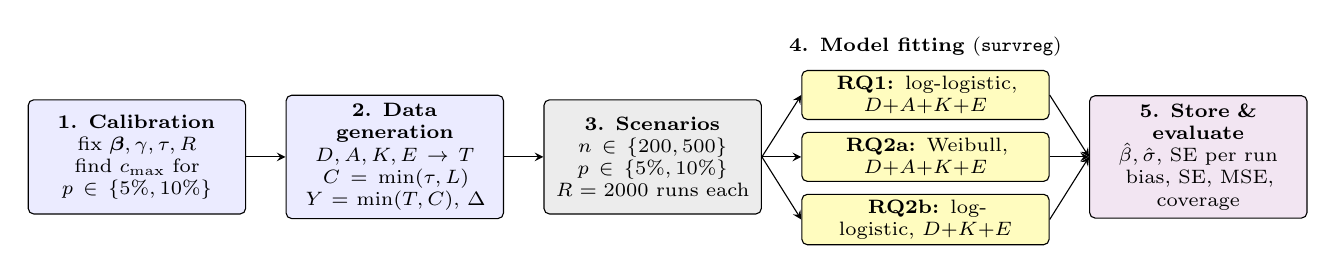
\begin{tikzpicture}[font=\scriptsize,>=stealth,node distance=5mm,
 box/.style={draw,rounded corners=2pt,align=center,inner sep=3pt,text width=2.55cm,minimum height=1.45cm},
 model/.style={draw,rounded corners=2pt,align=center,inner sep=2pt,text width=3.0cm,minimum height=0.5cm,fill=yellow!25}]
\node[box,fill=blue!8] (cal) {\textbf{1. Calibration}\\ fix $\boldsymbol\beta,\gamma,\tau,R$\\ find $c_{\max}$ for\\ $p\in\{5\%,10\%\}$};
\node[box,fill=blue!8,right=of cal] (gen) {\textbf{2. Data generation}\\ $D,A,K,E\to T$\\ $C=\min(\tau,L)$\\ $Y=\min(T,C)$, $\Delta$};
\node[box,fill=gray!15,right=of gen] (sc) {\textbf{3. Scenarios}\\ $n\in\{200,500\}$\\ $p\in\{5\%,10\%\}$\\ $R=2000$ runs each};
\node[model,right=of sc] (m2) {\textbf{RQ2a:} Weibull, $D{+}A{+}K{+}E$};
\node[model,above=1.5mm of m2] (m1) {\textbf{RQ1:} log-logistic, $D{+}A{+}K{+}E$};
\node[model,below=1.5mm of m2] (m3) {\textbf{RQ2b:} log-logistic, $D{+}K{+}E$};
\node[above=0.5mm of m1] {\textbf{4. Model fitting} (\texttt{survreg})};
\node[box,fill=violet!10,right=of m2] (out) {\textbf{5. Store \& evaluate}\\ $\hat\beta,\hat\sigma$, SE per run\\ bias, SE, MSE, coverage};
\draw[->] (cal) -- (gen);
\draw[->] (gen) -- (sc);
\foreach \m in {m1,m2,m3}{\draw[->] (sc.east) -- (\m.west); \draw[->] (\m.east) -- (out.west);}
\end{tikzpicture}
\caption{Simulation workflow: calibration of $c_{\max}$, data generation, the four scenarios, the three model fits and the evaluation.}\label{fig:flow}
\end{figure}
\vspace{-10pt}

\section{Performance measures}
We evaluate the estimates of $\beta_D,\beta_E,\beta_A,\beta_K$, with $\beta_E$ as the main target. In each of the $R=2000$ runs we store the estimate $\hat\beta$ and its standard error. With $\bar\beta$ the average estimate over all runs, we compute:
\textbf{Bias} $=\bar\beta-\beta$: is the estimate systematically wrong?
\textbf{Empirical SE} $=$ the standard deviation of the estimates: how much does the estimate vary between runs? (Variance $=\mathrm{SE}^2$.)
\textbf{MSE} $=$ the average of $(\hat\beta-\beta)^2\approx\mathrm{Bias}^2+\mathrm{Variance}$: the total error.
\textbf{Coverage} $=$ the share of 95\% confidence intervals that contain the true $\beta$: are the standard errors reliable? It should be close to 95\%.
For each scenario we also report the observed censoring rate and the number of runs that failed to converge (these are excluded). Both the log-logistic and the Weibull fits are AFT models fitted with \texttt{survreg}, so their coefficients are on the same scale and can be compared with the same true values. When age is left out, only $\beta_D,\beta_E,\beta_K$ are evaluated.

\section{Alternative (incorrect) analyses}
\textbf{(a) Wrong distribution: fitting a Weibull model.} We fit a Weibull AFT model instead of the log-logistic one. \emph{Why it is wrong:} the Weibull hazard can only increase, decrease or stay constant. It cannot rise and then fall, so it cannot capture the early ``dangerous peak'' in the true hazard.
\textbf{(b) Omitting an important covariate: leaving out age.} We fit the correct log-logistic model, but without age. \emph{Why it is wrong:} age is a confounder. It increases the number of comorbidities ($K$) and the chance of an extra-hepatic cause ($E$), and it also shortens survival directly.

\section{Hypotheses}
\textbf{RQ1: correct log-logistic model.}
\textbf{H1 (bias).} The estimated effects will be very close to the true values in all four scenarios, and any small bias at $n=200$ will be even smaller at $n=500$. The fitted model is the model that generated the data and censoring does not depend on the survival time, so the estimates are correct on average.
\textbf{H2 (sample size).} The empirical SE will drop by about one third and the MSE will fall to roughly 40\% of its value at $n=200$. More patients give more information, and with a bias close to zero the MSE is almost entirely variance.
\textbf{H3 (loss to follow-up).} Going from 5\% to 10\% loss will make the estimates slightly less precise but not biased, an effect much smaller than that of sample size. Extra random censoring only removes some observed events without pushing the estimates in a direction, and many patients are already censored at day 90.

\textbf{RQ2a: Weibull instead of log-logistic.}
\textbf{H4.} The Weibull model will clearly misestimate the intercept and the shape, while the covariate effects will be only slightly biased. The two models differ only in the assumed shape, so most of the misfit is absorbed by the intercept and shape. The Weibull hazard can only go up or down, so it cannot reproduce the early peak; because many patients are censored, the covariate effects will still be somewhat affected.
\textbf{H5.} The Weibull bias will not go away with more patients while its variance will, so it will look relatively worse at $n=500$ than at $n=200$. A wrong model precisely estimates the wrong thing: more data makes the estimate more stable but not more accurate.
\textbf{H6.} The Weibull model will be somewhat more biased at 10\% loss than at 5\%. With more censoring the estimates depend more on the assumed (wrong) shape of the distribution.

\textbf{RQ2b: leaving out the confounder age.}
\textbf{H7.} Comorbidities and damage outside the liver will look more harmful than they really are. In our data older patients have more comorbidities, more often have damage outside the liver and survive shorter, so without age part of its harmful effect is wrongly attributed to $K$ and $E$.
\textbf{H8.} The effect of days to treatment will stay close to its true value but be estimated slightly less precisely. Days to treatment was generated independently of age, so age does not confound it; the survival variation caused by age becomes unexplained noise, which reduces precision but does not push the estimates in a direction.

\newpage
\section{Results}
We ran the simulation from Part~II (seed 123, 2000 runs per scenario). The observed censoring was 43\% (5\% loss to follow-up) and 45\% (10\% loss). Table~\ref{tab:res} reports bias, empirical SE, MSE and coverage for $\beta_E$ and $\beta_K$ at 5\% loss; the 10\% loss results differ by less than 0.01 in SE. Figure~\ref{fig:res} shows the distribution of the estimates in all four scenarios.

\textbf{Correct analysis (M1).} Bias is between $-0.009$ and $+0.004$, coverage is 94--95\%, and the MSE of $\beta_E$ is 0.081 at $n=200$ and 0.030 at $n=500$.

\textbf{Incorrect analyses.} \emph{M2 (Weibull):} bias is $+0.08$ to $+0.10$ for $\beta_E$ and $+0.03$ to $+0.04$ for $\beta_K$; coverage is 87--92\%. \emph{M3 (no age):} bias is $-0.16$ to $-0.17$ for $\beta_E$ and $-0.12$ for $\beta_K$; coverage for $\beta_K$ is 78\% at $n=200$ and 54\% at $n=500$. For $\beta_D$ (not in the table), M3 has a bias below 0.001 and 94--95\% coverage.

\begin{table}[H]
\centering\scriptsize\setlength{\tabcolsep}{4pt}
\caption{Results at 5\% loss to follow-up over 2000 runs. SE = empirical standard error; Cov.\ = share of 95\% intervals that contain the true value.}\label{tab:res}
\begin{tabular}{@{}lr rrrr rrrr@{}}
\toprule
 & & \multicolumn{4}{c}{Etiology $\beta_E$ (true $-0.70$)} & \multicolumn{4}{c}{Comorbidities $\beta_K$ (true $-0.25$)} \\
\cmidrule(lr){3-6}\cmidrule(l){7-10}
Model & $n$ & Bias & SE & MSE & Cov. & Bias & SE & MSE & Cov. \\
\midrule
M1 (correct) & 200 & $-0.009$ & 0.284 & 0.081 & 95\% & $+0.001$ & 0.126 & 0.016 & 95\% \\
 & 500 & $+0.004$ & 0.173 & 0.030 & 95\% & $+0.001$ & 0.080 & 0.006 & 94\% \\
\addlinespace
M2 Weibull & 200 & $+0.078$ & 0.264 & 0.076 & 92\% & $+0.031$ & 0.122 & 0.016 & 91\% \\
 & 500 & $+0.097$ & 0.163 & 0.036 & 89\% & $+0.036$ & 0.078 & 0.007 & 87\% \\
\addlinespace
M3 no age & 200 & $-0.170$ & 0.276 & 0.105 & 90\% & $-0.124$ & 0.110 & 0.027 & 78\% \\
 & 500 & $-0.158$ & 0.169 & 0.053 & 86\% & $-0.124$ & 0.069 & 0.020 & 54\% \\
\bottomrule
\end{tabular}
\end{table}

\begin{figure}[H]
\centering
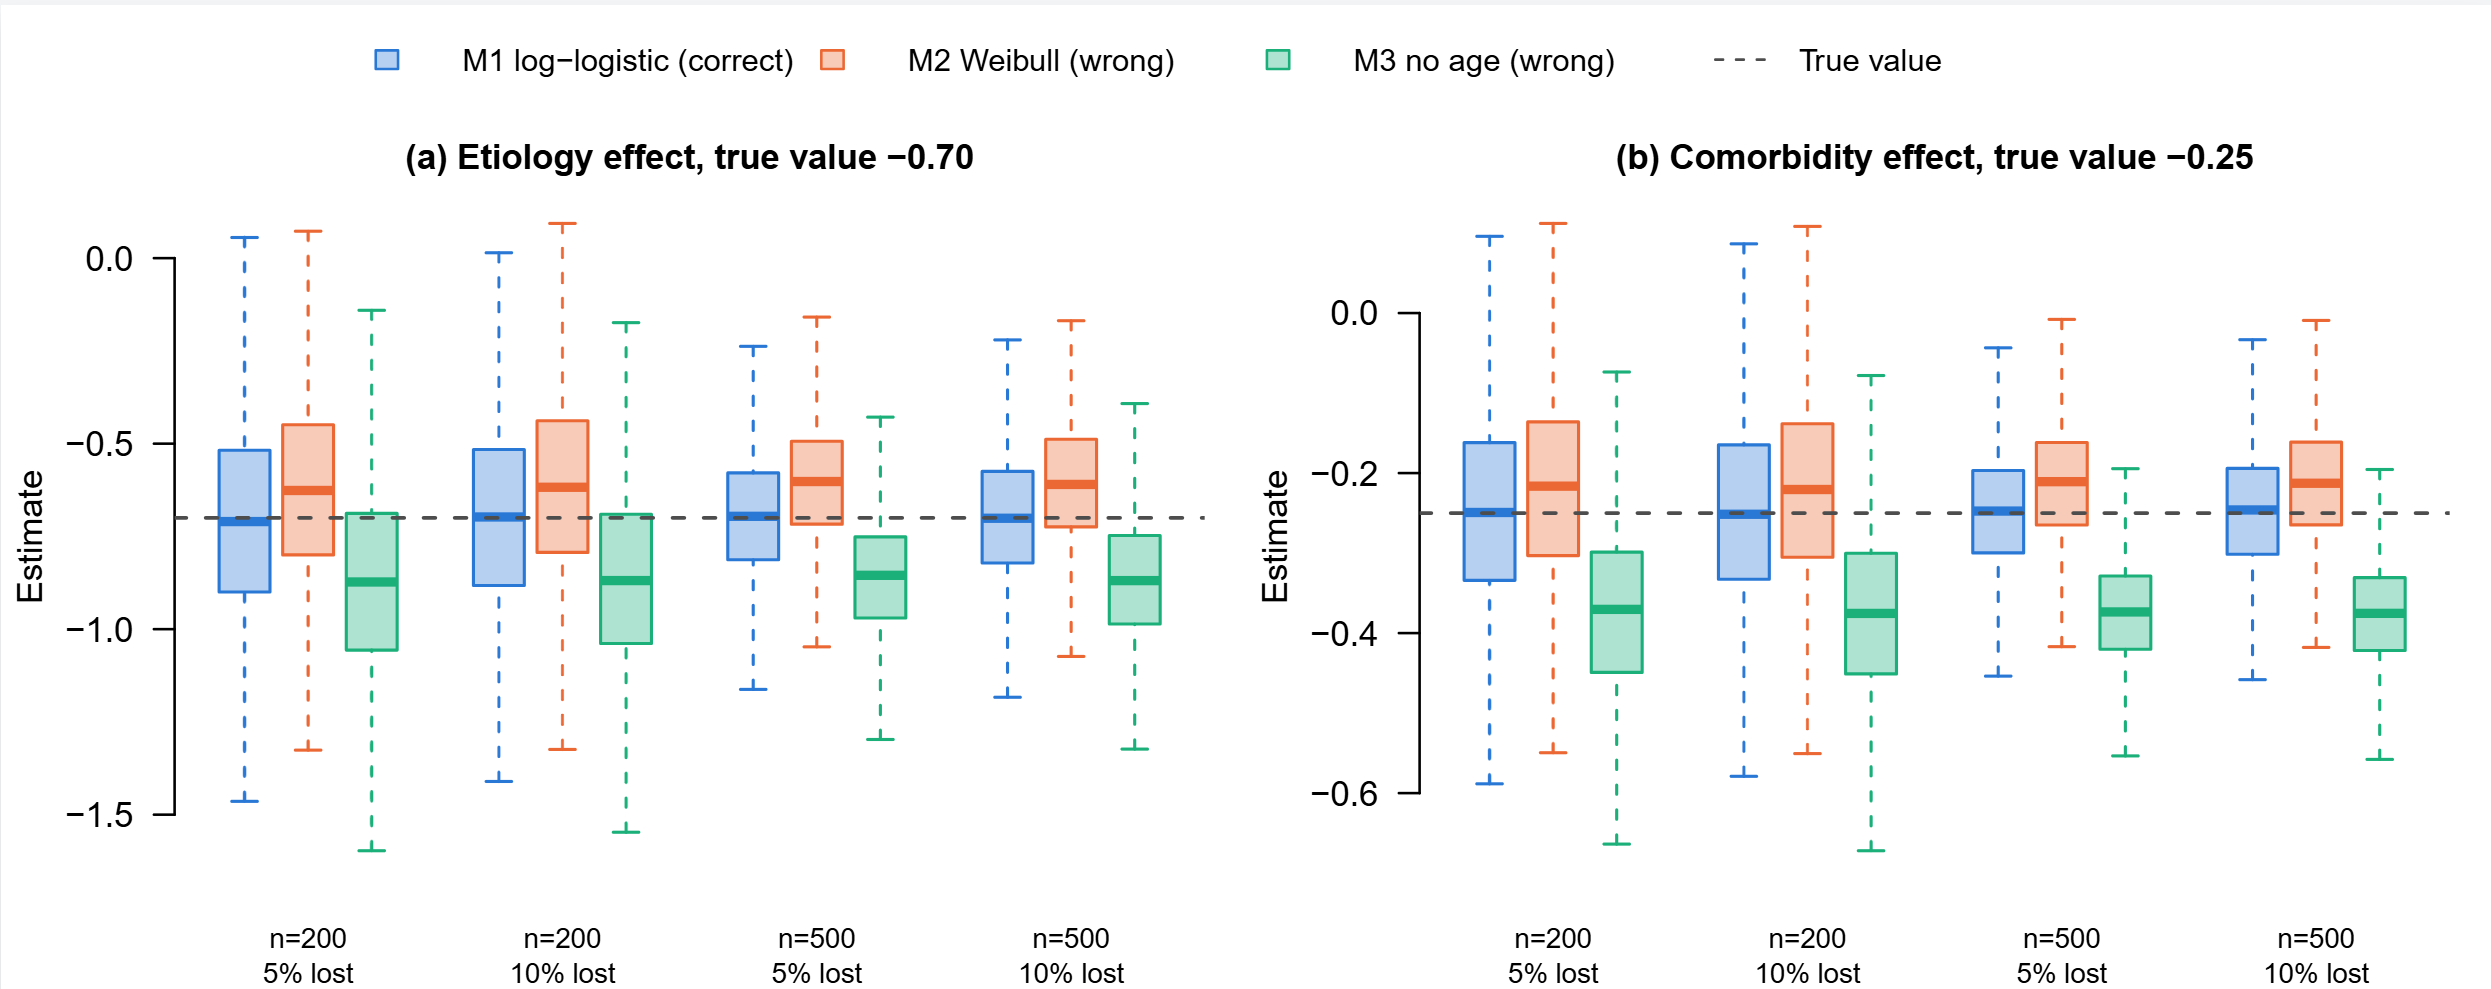
\includegraphics[width=0.8\linewidth]{image.png}
\caption{Estimates of $\beta_E$ and $\beta_K$ over 2000 runs (boxes: middle 50\%; dashed line: true value). Only M1 is centred on the truth.}\label{fig:res}
\end{figure}

\section{Evaluation}
\paragraph{RQ1}
\textbf{M1}:
\textbf{Bias}: the correctly specified log-logistic model is practically unbiased for both etiology ($\beta_E$ bias of $-0.009$ to $+0.004$) and comorbidities ($\beta_K$ bias of $+0.001$ to $+0.003$), and the same holds for $\beta_D$ and $\beta_A$, because the fitted model is the model that generated the data and censoring is independent of survival. Only the scale $\hat\sigma=1/\hat\gamma$ is slightly too small ($-0.015$ at $n=200$, $-0.008$ at $n=500$), the usual small-sample bias of maximum likelihood. \textbf{Variability}: SE decreases with the sample size ($\text{SE}_{\beta_E}$ drops from $0.284$ to $0.173$; $\text{SE}_{\beta_K}$ drops from $0.126$ to $0.080$), a factor of $0.61$ - $0.65$ that is close to the theoretical $\sqrt{200/500}=0.63$. Between 5\% and 10\% loss to follow-up the SE differs by less than $0.01$. The model based SEs match the empirical SEs, so the coverage stays at $94$ - $95$\%. \textbf{MSE}: since the bias is negligible, the MSE is almost entirely variance and falls with sample size($0.081$ to $0.030$ for $\beta_E$; $0.016$ to $0.006$ for $\beta_K$), to $37$--$42\%$ of its value at $n=200$. \textbf{Practical implications}: with 43\% - 45\% censoring , the correct model already gives unbiased estimates and valid confidence intervals at $n = 200$, but they are wide: the 95\% interval for the etiology time ratio ($e^{\beta_E}=0.50$) runs from $0.28$ to $0.87$ at $n=200$ and from $0.35$ to $0.70$ at $n=500$. The precision of the results is determined by the sample size, not by a moderate amount of extra loss to follow-up.
\paragraph{RQ2}
\textbf{M2}:
\textbf{Bias}: Weibull introduces a positive bias for both etiology ($\beta_E$ bias of $+0.078$ to $+0.097$) and comorbidities ($\beta_K$ bias of $+0.031$ to $+0.036$), because a monotonic Weibull hazard cannot capture the early "dangerous peak" of the true log-logistic hazard. \textbf{Variability}: SE decreases with n ($\text{SE}_{\beta_E}$ drops from $0.264$ to $0.163$; $\text{SE}_{\beta_K}$ drops from $0.122$ to $0.078$). \textbf{MSE}: random sampling variance dominates at $n=200$, where M2’s slightly smaller SE yields a lower MSE for $\beta_E$ than M1 ($0.076$ vs. $0.081$). However, at $n=500$, as variance decreases, M2’s bias makes its MSE worse than M1 ($0.036$ vs. $0.030$ for $\beta_E$; $0.007$ vs. $0.006$ for $\beta_K$).  \textbf{Practical implications}: misspecifying the baseline hazard causes the clinicians to underestimate the survival impact of etiology and comorbidities.


\textbf{M3}:
\textbf{Bias}: Omitting the age introduces a negative bias for both etiology ($\beta_E$ bias of $-0.170$ to $-0.158$) and comorbidities ($\beta_K$ bias of $-0.124$ across both sample sizes). Because older age increases both the likelihood of $E$ and $K$ while also shortening survival, leaving age out of the model forces $\hat{\beta}_E$ and $\hat{\beta}_K$ to increase their effect. $\beta_D$ remains unbiased (bias $<0.001$) because it is independent of age. \textbf{Variability}: SE decreases with n ($\text{SE}_{\beta_E}$ drops from $0.276$ to $0.169$; $\text{SE}_{\beta_K}$ drops from $0.110$ to $0.069$) and differs by less than $0.01$ between $5\%$ and $10\%$ loss to follow-up. \textbf{MSE}: remains worse than in M1 for both $n=200$ ($0.105$ vs. $0.081$ for $\beta_E$; $0.027$ vs. $0.016$ for $\beta_K$) and $n=500$ ($0.053$ vs. $0.030$ for $\beta_E$; $0.020$ vs. $0.006$ for $\beta_K$), where squared bias strongly influences the total error. \textbf{Practical implications}: failing to adjust for a clinical confounder like age, it strongly increases the harmful survival impact of etiology and comorbidities, leading to misguiding clinical risk assessments.


\section{Comparison with expectations}
\subsection{RQ1}
\textbf{H1: True}: All biases of M1 are below $0.01$ in absolute value and coverage is close to 95\% in every scenario. The biases are already so small at $n=200$ that they are mostly simulation noise, so they do not visibly shrink further at $n=500$; the small bias of the scale does shrink ($-0.015$ to $-0.008$), as predicted.

\textbf{H2: True)}: We predicted that the SE would drop by about one third and the MSE would fall to about 40\%. The observed SE ratios are $0.61$--$0.65$ and the MSE ratios $0.37$--$0.42$ for all four coefficients, because with a correct model and negligible bias the precision follows the $1/\sqrt n$ rule.

\textbf{H3: Partly True}: As expected, 10\% loss introduces no bias and has a much smaller effect than sample size. However, the predicted small loss of precision does not appear: the SEs at 10\% loss are sometimes larger and sometimes smaller than at 5\%, within simulation noise. This is because the extra loss barely reduces the number of observed events: total censoring rises only from 42.9\% to 44.6\% (Table~\ref{tab:censoring}), since many of the extra lost patients would have been censored at day 90 anyway.

\subsection{RQ2}
\textbf{H4: True!} M2 slightly biased the covariate estimates ($\beta_E$ bias of $+0.08$ to $+0.10$; $\beta_K$ bias of $+0.03$ to $+0.04$). Because the Weibull hazard is strictly monotonic, it cannot reproduce the early "dangerous peak". While the intercept and shape parameters absorb most of this mismatch, the high censoring rate ($43\text{--}45\%$) causes the misspecification to slightly bias the covariate effects.
\textbf{H5: True!} M2 bias persisted for n=500 and worsened the coverage. Bias remained +0.97, but coverage dropped from 92\% to 89\%. The misspecified model fits to the wrong parameter value. Growing n would reduce SE around the biased value, shifting the center of the coverage.
\textbf{H6: False!} M2 was less biased for a loss of 10\% compared to 5\%. The results differ by less than 0.01 in SE. Doubling the random loss from 5\% only increased the total observed censoring from 43\% to 45\% being insignificant.
\textbf{H7: True!} M3 produced a large negative effect on $\beta_E$ (from -0.170 to -0.158) and $\beta_K$ (-0.124). The older age increases both the probability of $E$ and $K$ while also reducing the survival time. Leaving out this confounder would make $\hat{\beta}_E$ and $\hat{\beta}_K$ to strongly increase the harmful impact caused by them.
\textbf{H8: True!} In M3, the effect of days to treatment ($\hat{\beta}_D$) had a bias below $0.001$ and maintained $94\text{--}95\%$ coverage. $D$ was generated independently of $A$, hence it is not a confounder for $D$.

\section{Conclusions}

\section{Limitations}
We have noticed the following limitations in our study:
\begin{itemize}
    \item The parameters $\beta$, $\gamma$ are assumed, not estimated, and the covariate distributions are reasonable guesses, which may work for this scenario, but may not apply to real-life cases and datasets.
    \item Covariates are simplistic, with no interactions or relations between them (i.e. age and etiology), assumes no changes in covariates over time (i.e. an increase in K due to other health issues).
    \item Limited scope with only 200 or 500 subjects, for a maximum of 2000 runs each and the same $\beta$ and $\gamma$ values, may lead to biases.
    \item Covariate K is overly-simplistic, different comorbidities and issues may have different effects over the patients, so just counting them assumes that they have an equal effect, i.e. diabetes is considered as damaging as an auto-immune disease.
\end{itemize}


%=====================================================================
\newpage
\section*{Use of AI tools}
\todo{}


\section*{Contribution statement}
\begin{itemize}[leftmargin=1.2em,itemsep=2pt]
\item Avram Andrei: \todo{}
\item Mihaiescu Cristian: \todo{}
\item Szelestey Adam: \todo{}
\item Vrincianu Darius: \todo{}
\item Zeng Qin Tao: Results (performance measures code, tables and figure).
\end{itemize}
All group members confirm that this contribution statement is accurate.

\section*{References}
\begin{itemize}[leftmargin=1.2em,itemsep=2pt]\small
\item Chris-Olaiya, A., Kapoor, A., Ricci, K. S., \& Lindenmeyer, C. C. (2021). Therapeutic plasma exchange in liver failure. \emph{World Journal of Hepatology}, 13(8), 904--915.
\item Huang, D. Q., Terrault, N. A., Tacke, F., et al. (2023). Global epidemiology of cirrhosis --- aetiology, trends and predictions. \emph{Nature Reviews Gastroenterology \& Hepatology}, 20(6), 388--398.
\item Jepsen, P. (2014). Comorbidity in cirrhosis. \emph{World Journal of Gastroenterology}, 20(23), 7223--7230.
\item Larsen, F. S., et al. (2016). High-volume plasma exchange in patients with acute liver failure: An open randomised controlled trial. \emph{Journal of Hepatology}, 64(1), 69--78.
\item Alexander, E. C., \& Deep, A. (2022). Therapeutic plasma exchange in children with acute liver failure (ALF): Is it time for incorporation into the ALF armamentarium? \emph{Pediatric Nephrology}, 37(8), 1775--1788.
\end{itemize}

\newpage
\section{Appendix}
\section*{Software implementation}
Condensed R code (left: data generation and censoring; right: model fitting and storage).\\[2pt]
\begin{minipage}[t]{0.49\textwidth}
\begin{lstlisting}[style=rcode]
set.seed(123)
beta <- c(b_0 = 5.8, b_d = -0.1, b_a = -0.02,
          b_k = -0.25, b_e = -0.7)
gamma_val <- 1.1; tau <- 90; sim_runs <- 2000
loss_vec <- c(0.05, 0.10)

generate_data <- function(m) {          # covariates
  d <- rgamma(m, shape = 2, scale = 2)
  a <- pmin(pmax(rnorm(m, 45, 15), 18), 85)
  k <- rpois(m, exp(-2.75 + 0.05 * a))
  e <- rbinom(m, 1, plogis(-3.9 + 0.06 * a))
  data.frame(days = d, age = a, nr_comor = k, damage = e)
}
draw_t <- function(x, beta, gamma_val) { # event times
  lambda <- exp(beta["b_0"] + beta["b_d"] * x$days +
    beta["b_a"] * x$age + beta["b_k"] * x$nr_comor +
    beta["b_e"] * x$damage)
  u <- runif(nrow(x))
  lambda * (u / (1 - u))^(1 / gamma_val)
}
# calibrate c_max: P(L < min(T, tau)) = target loss
find_cmax <- function(target, m, cutoff) {
  times <- draw_t(generate_data(m), beta, gamma_val)
  min_t <- pmin(times, cutoff)
  f <- function(cm) mean(pmin(min_t, cm) / cm) - target
  uniroot(f, c(5, max(times)), tol = 0.5)$root
}
cmax <- lapply(loss_vec, find_cmax, m = 1e6, cutoff = tau)

generate_cohort <- function(n, runs, cmax) {
  m <- n * runs                       # all runs at once
  x <- generate_data(m)
  t_event <- draw_t(x, beta, gamma_val)
  cens <- pmin(tau, runif(m, 0, cmax))  # C = min(tau, L)
  stat <- as.integer(t_event <= cens)
  rid  <- rep(seq_len(runs), each = n)
  c_n  <- tapply(1L - stat, rid, sum)   # per-run censor count
  data.frame(run_id = rid, x,
             time = pmin(t_event, cens), status = stat,
             censored = as.integer(c_n[rid]))
}
simulated_data <- list(
  n200_loss05 = generate_cohort(200, sim_runs, cmax[[1]]),
  n200_loss10 = generate_cohort(200, sim_runs, cmax[[2]]),
  n500_loss05 = generate_cohort(500, sim_runs, cmax[[1]]),
  n500_loss10 = generate_cohort(500, sim_runs, cmax[[2]]))
saveRDS(simulated_data, "simulated_data.rds")
\end{lstlisting}
\end{minipage}\hfill
\begin{minipage}[t]{0.49\textwidth}
\begin{lstlisting}[style=rcode]
library(survival)
simulated_data <- readRDS("simulated_data.rds")

# Per-run empirical loss to follow-up and total censoring
loss_run <- lapply(simulated_data, function(d)
  tapply(d$status == 0 & d$time < 90, d$run_id, mean))
cens_run <- lapply(simulated_data, function(d)
  tapply(d$status == 0, d$run_id, mean))
censoring_summary <- data.frame(
  loss_mean = vapply(loss_run, mean, numeric(1)),
  loss_sd   = vapply(loss_run, sd, numeric(1)),
  cens_mean = vapply(cens_run, mean, numeric(1)),
  cens_sd   = vapply(cens_run, sd, numeric(1)))

fit_one_run <- function(d, formula, dist) {
  fit <- tryCatch(survreg(formula, data = d, dist = dist),
                  error = function(e) NULL,
                  warning = function(w) NULL)
  if (is.null(fit)) return(NULL)  # failed / no convergence
  se <- sqrt(diag(vcov(fit)))[names(coef(fit))]
  c(coef(fit), scale = fit$scale,
    setNames(se, paste0("se_", names(se))))
}
fit_model_across_runs <- function(df, formula, dist) {
  est <- lapply(split(df, df$run_id), fit_one_run,
                formula, dist)
  failed <- vapply(est, is.null, logical(1))
  out <- as.data.frame(do.call(rbind, est[!failed]))
  attr(out, "n_failed") <- sum(failed)
  out
}
f_full   <- Surv(time, status) ~ days + age + nr_comor + damage
f_no_age <- Surv(time, status) ~ days + nr_comor + damage
fit_all <- function(f, dist)
  lapply(simulated_data, fit_model_across_runs, f, dist)

model_estimates <- list(
  rq1_loglogistic = fit_all(f_full, "loglogistic"),
  rq2a_weibull    = fit_all(f_full, "weibull"),
  rq2b_no_age     = fit_all(f_no_age, "loglogistic"),
  censoring_summary = censoring_summary)
saveRDS(model_estimates, "model_estimates.rds")
\end{lstlisting}
\end{minipage}

\section*{Response to Feedback}
\textbf{Feedback received:} ``Report the mean value of the censoring ratio and the standard deviation across runs for each simulation scenario ($n=200, n=500$; 5\%, 10\%).''

\textbf{How it was addressed:} Censoring in our simulation comprises two distinct mechanisms: (i) random uninformative loss to follow-up prior to study conclusion ($L \sim \text{Unif}(0, c_{\max})$ with $L < \min(T, \tau)$), calibrated to 5\% and 10\%; and (ii) administrative censoring at the $\tau = 90$-day study horizon ($T \ge 90$). For each run across all $R=2000$ simulation runs per scenario, we evaluated both the empirical loss to follow-up rate ($\text{status}=0 \land \text{time} < 90$) and the total composite censoring ratio ($\text{status}=0$).

As shown in Table~\ref{tab:censoring}, empirical loss to follow-up closely matches our calibration targets ($5.00\% \pm 1.54\%$ and $10.04\% \pm 2.08\%$ for $n=200$; $5.01\% \pm 0.96\%$ and $10.04\% \pm 1.39\%$ for $n=500$). Administrative censoring accounts for the remaining censored cases ($\sim 37.8\%$ in the 5\% scenario; $\sim 34.5\%$ in the 10\% scenario), yielding overall composite censoring proportions of approximately 42.8\% and 44.6\%. The across-run standard deviations decrease by a factor of $\sqrt{500/200}\approx 1.58$ from $n=200$ to $n=500$, as expected from binomial sampling variability. Both summary metrics have been integrated into the simulation outputs in \texttt{hw2\_model\_fitting.R}.

\begin{table}[H]
\centering\footnotesize
\caption{Empirical loss to follow-up and total censoring ratio across 2000 simulation runs (mean and std).}\label{tab:censoring}
\begin{tabular}{@{}cccccc@{}}
\toprule
& & \multicolumn{2}{c}{Empirical Loss to Follow-up} & \multicolumn{2}{c}{Total Censoring Ratio} \\
\cmidrule(lr){3-4} \cmidrule(lr){5-6}
Sample size ($n$) & Target Loss & Mean & Std. Dev. & Mean & Std. Dev. \\
\midrule
200 & 5\%  & 0.0500 (5.0\%)  & 0.0154 (1.5\%) & 0.4286 (42.9\%) & 0.0351 (3.5\%) \\
200 & 10\% & 0.1004 (10.0\%) & 0.0208 (2.1\%) & 0.4456 (44.6\%) & 0.0357 (3.6\%) \\
\addlinespace
500 & 5\%  & 0.0501 (5.0\%)  & 0.0096 (1.0\%) & 0.4273 (42.7\%) & 0.0220 (2.2\%) \\
500 & 10\% & 0.1004 (10.0\%) & 0.0139 (1.4\%) & 0.4452 (44.5\%) & 0.0227 (2.3\%) \\
\bottomrule
\end{tabular}
\end{table}
\vspace{-6pt}

\end{document}
